\documentclass[a4paper]{article}
\usepackage{graphicx}
\usepackage{amsmath, amsfonts, geometry, float, listings, enumerate, multicol}
\usepackage{multicol, float, color, colortbl}
\usepackage{tikz, titlesec, parskip}

\titlespacing{\section}{0pt}{10pt}{0pt}
\titlespacing{\subsection}{0pt}{10pt}{0pt}
\titlespacing{\subsubsection}{0pt}{10pt}{0pt}

\usetikzlibrary{calc,patterns,through}
\newcommand{\arcangle}{%
	\mathord{<\mspace{-9mu}\mathrel{)}\mspace{2mu}}%
}

\renewcommand{\baselinestretch}{1.2}
\geometry{
	a4paper,
	total={170mm,257mm},
	left=20mm,
	top=20mm,
}
\usepackage{fancyhdr}
\pagestyle{fancy}
\fancyhf{}
\rhead{\textbf{سیگنال‌ها و سیستم‌ها}}
\lhead{\textbf{تمرین تئوری سری دوم}}
\cfoot{(\space \space \space \space \textbf{\thepage}  \space \space \space)}
\renewcommand{\headrulewidth}{1pt}
\renewcommand{\footrulewidth}{1pt}

\usepackage{xepersian}
%\setlatintextfont{Times New Roman}
\settextfont{XB Niloofar}
\setdigitfont{XB Niloofar}
\DefaultMathsDigits
\usepackage{amsmath}
\usepackage{pgfplots}
\tikzset{declare function={unitstep(\x)=notless(\x,0);}}
\tikzset{declare function={delta(\x)=equal(\x,0);}}

\begin{document}
	\begin{minipage}{0.6\textwidth}
		
		\begin{center}
			\begin{bf}
				باسمه تعالی\\
				\vspace{0.25cm}
				دانشگاه صنعتی شریف\\
				\vspace{0.25cm}
				دانشکده مهندسی برق\\
				\vspace{0.5cm}
				
				\large
				25742 گروه ۴ - سیگنال‌ها و سیستم‌ها - بهار ۱۳۹۷-۹۸\\
				\Large
				\vspace{0.4cm}
				تمرین تئوری سری دوم\\
				\vspace{0.3cm}
			\end{bf}
			\small{موعد تحویل: شنبه یازدهم اسفند ماه، ابتدای کلاس}
			
			
		\end{center}
		\normalsize
	\end{minipage} \hfill
	\begin{minipage}{0.35\textwidth}
		
		\begin{flushleft}
			
\includegraphics[width=0.6\textwidth]{Shariflogo.png}\\ \large
		\end{flushleft}
		
	\end{minipage}
	\\
	
	\rule[0.1\baselineskip]{\textwidth}{1.5pt}
	\textbf{
		توجه: تنها تمارینی که با علامت
		\textcolor{red}{$\ast$}
		مشخص شده‌اند، تحویل گرفته شده و تصحیح می‌شوند.}\\
	\rule[0.1\baselineskip]{\textwidth}{1.5pt}\par
	
	\large
	
	\section{ \textcolor{red}{$\ast$} 
		خواص کانولوشن (۱۵ نمره)
	}
	\begin{enumerate}
		\item 
		یک سیستم پیوسته-زمان به صورت 
		$y(t) = x(t)*h(t)$	
		در نظر بگیرید. نشان دهید پاسخ این سیستم به ورودی 
		$\frac{dx}{dt}$
		برابر
		$\frac{dy}{dt}$
		است. 
		
		\item
		یک سیستم گسسته-زمان به صورت  
		$y[n] = x[n]*h[n]$	
		در نظر بگیرید. نشان دهید:
		$$\sum_{n=-\infty}^{\infty}y[n] = 
		\Big(\sum_{n=-\infty}^{\infty}x[n]\Big)\Big(\sum_{n=-\infty}^{\infty}h[n]\Big)
		$$
		
		\item 
		یک سیستم پیوسته-زمان به صورت 
		$y(t) = x(t)*h(t)$
		در نظر بگیرید. نشان دهید اگر 
		$x(t)$
		با تناوب $T$ متناوب باشد، آن‌گاه $y(t)$  نیز با همین دوره‌ی تناوب، تناوبی است.
		
	\end{enumerate}
	
	\section{ \textcolor{red}{$\ast$} 
		کانولوشن به صورت ماتریسی
		(۱۵ نمره)
	}
	\begin{itemize}
		\item
		فرض کنید سیگنال $x[n]$،  تنها در بازه‌ی 
		$0\leq n <M$
		و سیگنال $h[n]$، تنها در بازه‌ی 
		$0\leq n <N$
		ناصفر باشند. بازه‌‌ای که سیگنال 
		$y[n] = x[n]*h[n]$
		در آن ناصفر است را بیابید.
		\item
		پاسخ بخش قبل را یک‌بار به کمک محاسبه‌ی تحلیلی و یک‌بار به کمک استدلال گرافیکی برای سیگنال‌های 
		$x[n] = u[n] - u[n-5]$
		و
		$h[n] = 2u[n] - 2u[n-2]$
		بررسی کنید.
		
		\item
		فرض کنید سیگنال   $x[n]$ در خارج بازه‌ی  
		$n = 0, 1,...,L-1$
		و 
		سیگنال 
		$h[n]$
		در خارج بازه‌ی 
		$n = 0, 1,...,M-1$
		صفر باشد. فرض کنید 
		$y[n] = x[n] * h[n]$.
		می‌دانیم که طول سیگنال $y[n]$ نیز محدود است. بگیرید:
		$$\mathbf{X} = \Big[x[0], x[1],..., x[L-1]\Big]$$
		و 
		$$\mathbf{Y} = \Big[y[0], y[1],..., y[\textrm{حد بخش اول}]\Big]$$
		ماتریس 
		$\mathbf{H}$
		را به نحوی بیابید که 
		$\mathbf{Y} = \mathbf{H}\mathbf{X}$.
		
	\end{itemize}
	
	\newpage
	\section{
		خواص سیستم‌ها (۱۵ نمره)
	}
	برای هر یک از سیستم‌های 
	\lr{LTI}،
	با پاسخ ضربه‌ی داده‌شده،  علّی بودن/نبودن و پایدار بودن/نبودن را بررسی کنید.
	\begin{latin}
		\begin{itemize}
			\item  \textcolor{red}{$\ast$}  $h_1[n] = (\frac{1}{2})^n u[-n]$
			\item  \textcolor{red}{$\ast$}  $h_2[n] = (-\frac{1}{2})^n u[n] + (1.01)^n u[n-1]$
			\item  \textcolor{red}{$\ast$}  $h_3(t) = e^{2t} u(-1-t)$
			\item $h_4(t) = te^{-t}u(t)$
			\item  \textcolor{red}{$\ast$}  $h_5[n] = \sum_{p = -1}^{\infty} \delta[n-2p]$
			\item  \textcolor{red}{$\ast$}  $h_6(t) = \cos(\pi t)$
			\item $h_7[n] = (-1)^n u[-n]$
		\end{itemize}
	\end{latin}
	
	
	\section{
		\textcolor{red}{$\ast$}
		شناسایی سیستم (۱۵ نمره)
	}
	اگر پاسخ یک سیستم 
	\lr{LTI}
	به ورودی
	$x_0[n]$
	برابر 
	$y_0[n]$
	باشد، پاسخ این سیستم به 
	$x_1[n]$
	را بیابید.
	\begin{center}
		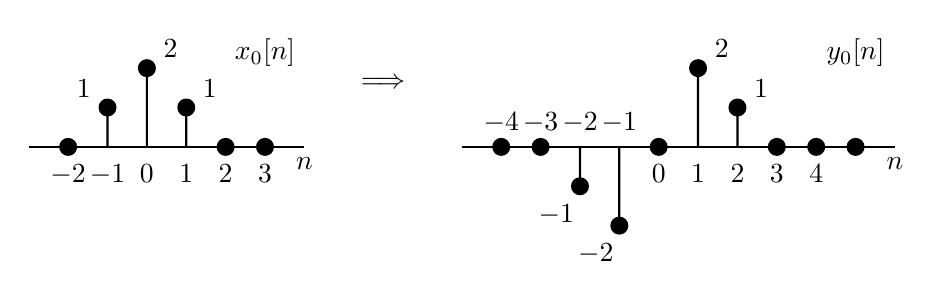
\begin{tikzpicture}[thick,scale=0.5]
		\draw[-] (-3,0) -- (4,0) node [below] {$n$};
		\foreach \x in {-2,...,3}
		{\draw[fill=black] (\x,0) -- (\x,{delta(\x-1)+2*delta(\x)+delta(\x+1)}) circle (0.2cm);
			\draw (\x,-0.2) node[below] {$\x$};
		}
		\draw (-1-0.6,1) node[above] {$1$};
		\draw (0.6,2) node[above] {$2$};
		\draw (1+0.6,1) node[above] {$1$};
		
		\draw (3,3) node[below] {$x_0[n]$};
		\draw (6,2) node[below] {$\Longrightarrow$};
		\draw[-] (8,0) -- (19,0) node [below] {$n$};
		\foreach \x in {9,...,18}
		{\draw[fill=black] (\x,0) -- (\x,{-delta(\x-11)-2*delta(\x-12)+2*delta(\x-14)+delta(\x-15)}) circle (0.2cm);
		}
		\foreach \x in {-4,...,-1}
		{
			\draw (\x+13,0.1) node[above] {$\x$};
		}
		\foreach \x in {0,...,4}
		{
			\draw (\x+13,-0.2) node[below] {$\x$};
		}
		\draw (18,3) node[below] {$y_0[n]$};
		\draw (11-0.6,-1-0.2) node[below] {$-1$};
		\draw (12-0.6,-2-0.2) node[below] {$-2$};
		\draw (14+0.6,2) node[above] {$2$};
		\draw (15+0.6,1) node[above] {$1$};
		\end{tikzpicture}
	\end{center}
	\begin{center}
		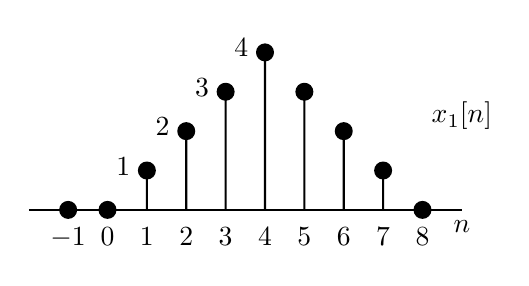
\begin{tikzpicture}[thick,scale=0.5]
		\draw[-] (-2,0) -- (9,0) node [below] {$n$};
		\foreach \x in {-1,...,8}
		{\draw[fill=black] (\x,0) -- (\x,{delta(\x-1) + 2*delta(\x-2) + 3*delta(\x-3) + 4*delta(\x-4) + 3*delta(\x-5) + 2*delta(\x-6) + delta(\x-7)}) circle (0.2cm);
			\draw (\x,-0.2) node[below] {$\x$};
		}
		\draw (9,3) node[below] {$x_1[n]$};
		\foreach \x in {1,...,4}{
			\draw (\x-0.6,\x+0.6) node[below] {$\x$};
		}
		\end{tikzpicture}
	\end{center}
	
	
	\section{
		\textcolor{red}{$\ast$}
		توابع همبستگی (۱۵ نمره)
	}
	تابع همبستگی متقابل بین دو سیگنال حقیقی $x(t)$ و $y(t)$  به صورت 
	$$R_{xy}(t) = \int_{-\infty}^{\infty}x(\tau)y(\tau-t)d\tau$$
	
	تعریف می‌شود. 
	
	الف) نشان دهید که  
	$R_{xy}(t) = x(t) * y(-t)$.
	
	ب)  نشان دهید
	$R_{xy}(t) = R_{yx}(-t)$.
	
	
	ج) خود همبستگی بین سیگنال‌های 
	$x(t) = u(t) - 2u(t-1) + u(t-2)$
	و
	$y(t) = u(t+1) - u(t)$
	را به دست آورید.
	
	د) سیستمی را در نظر بگیرید که  خروجی آن، تابع همبستگی ورودی  با خود ورودی است. آیا این سیستم خطی است؟ تغییرناپذیر با زمان چطور؟
	
	\section{
		\textcolor{red}{$\ast$}
		حذف اکو‌های سیگنال (۱۰ نمره)
	}
	یکی از کاربرد‌های سیستم‌های خطی و تغییرناپذیر با زمان، از بین بردن «اعوجاج» در سیگنال‌هاست. یک مثال از این کاربرد‌ها، حذف اکو‌ از سیگنال‌های صوتی است. 
	
	سیستمی را با پاسخ‌ ضربه‌ی ‌ زیر در نظر بگیرید.
	$$h(t) = \sum_{k = 0}^{\infty}h_k \delta(t-kT)$$
	بعد از عبور سیگنال صوتی 
	$x(t)$
	از این سیستم، اکو‌هایی با فاصله‌ی $T$ از سیگنال با آن جمع می‌شوند.
	
	فرض کنید سیگنال 
	$x(t)$،
	یک سیگنال صوتی باشد. این سیگنال  از سیستم $h$ عبور کرده و به دست ما می‌رسد. یعنی سیگنال
	$x_1(t) = x(t)*h(t)$
	را در اختیار داریم. می‌خواهیم با عبور سیگنال
	$x_1(t)$
	از سیستمی دیگر با پاسخ ضربه‌ی 
	$$g(t) = \sum_{k = 0}^{\infty}g_k \delta(t-kT)$$
	به سیگنال 
	$x(t)$
	برسیم. ضرایب 
	$g_k$
	را بر حسب
	$h_k$
	به دست آورید. در درسی سیستم‌های مخابراتی، به صورت مفصل در مورد سیستم‌های حذف اکو بحث خواهد شد.
	\section{دیاگرام بلوکی}
	پاسخ ضربه‌ی سیستم زیر را بر حسب پاسخ ضربه‌ی زیر-سیستم‌های آن به دست آورید.
	\begin{figure}[h!]
		\centering
		\includegraphics[scale=0.45]{subsys.png}
	\end{figure}
	
	\section{بی‌نام}
	شرطی لازم و کافی بیابید به نحوی که برای هر ورودی 
	$x[n]$،
	به سیستم 
	$y[n] = h[n] * x[n]$
	داشته باشیم:
	$$\forall n: \;\; \max\{|x[n]|\}\geq\max\{|y[n]|\}.$$
	\newpage
	\section{
		\textcolor{red}{$\ast$}
		بررسی سیستم‌های تک‌قطبی (۱۵ نمره)
	}
	یک سیستم خطی و تغییرناپذیر با زمان، با پاسخ ضربه‌ی 
	$h[n] = a^n u[n]$
	در نظر بگیرید.
	\begin{itemize}
		\item 
		پاسخ این سیستم را به ورودی 
		$x_1[n] = e^{j\pi n/2}$
		محاسبه کنید.
		\item 
		به کمک  بخش قبل، پاسخ این سیستم را به ورودی 
		$x_2[n] = \cos(n\pi/2)$
		به دست آورید.
		\item 
		پاسخ این سیستم به ورودی 
		$x_3[n] =e^{j\pi n/2} u[n] $
		محاسبه کنید.
		\item
		برای $n$های بزرگ، پاسخ به $x_3$ و $ x_1$
		را مقایسه کنید.
	\end{itemize}
	
	\section{
		محاسبه‌ی کانولوشن
	}
	کانولوشن سیگنال‌های داده‌‌شده‌ی زیر را محاسبه کنید.
	\begin{latin}
		\begin{itemize}
			
			\item 
			
			$x[n] = \alpha^n u[n]$\\
			$y[n] = \beta^n u[n]$
			\item
			$x(t) = u(t) - 2u(t-2) + u(t-5)$\\
			$h(t) = e^{2t}u(1-t)$
			\item
			\item
			\begin{figure}[h]
				\centering
				\includegraphics[scale=0.45]{۱.png}
			\end{figure}
			
			\item
			\begin{figure}[h]
				\centering
				\includegraphics[scale=0.5]{۴.png}
			\end{figure}
			\item
			\begin{figure}[h]
				\centering
				\includegraphics[scale=0.45]{۵.png}
			\end{figure}
		\end{itemize}
	\end{latin}
	
	
	\section{تمارین منتخب از کتاب}
	\begin{latin}
		\textbf{Problems of Chapter 2:}\\
		Sec. 2.1 – [44b,c] (DT signals and convolution) \\
		Sec. 2.2 – [44a,d, 47, 71] (CT signals and convolution) \\
		Sec. 2.3 – [48, 49, 51, 28, 29, 34, 35, 36] (system properties)\\
		Sec. 2.4 – [53, 58, 54, 55, 56, 59] (Differential and difference equations) \\
		Sec. 2.5 – [69, 71]
	\end{latin}
\end{document}